% This is a fun drawing of a spiral Galaxy using the tikz library.

\documentclass[tikz,border=10pt]{standalone}
\usepackage{tikz}
\usetikzlibrary{math} % For random number generation

\begin{document}
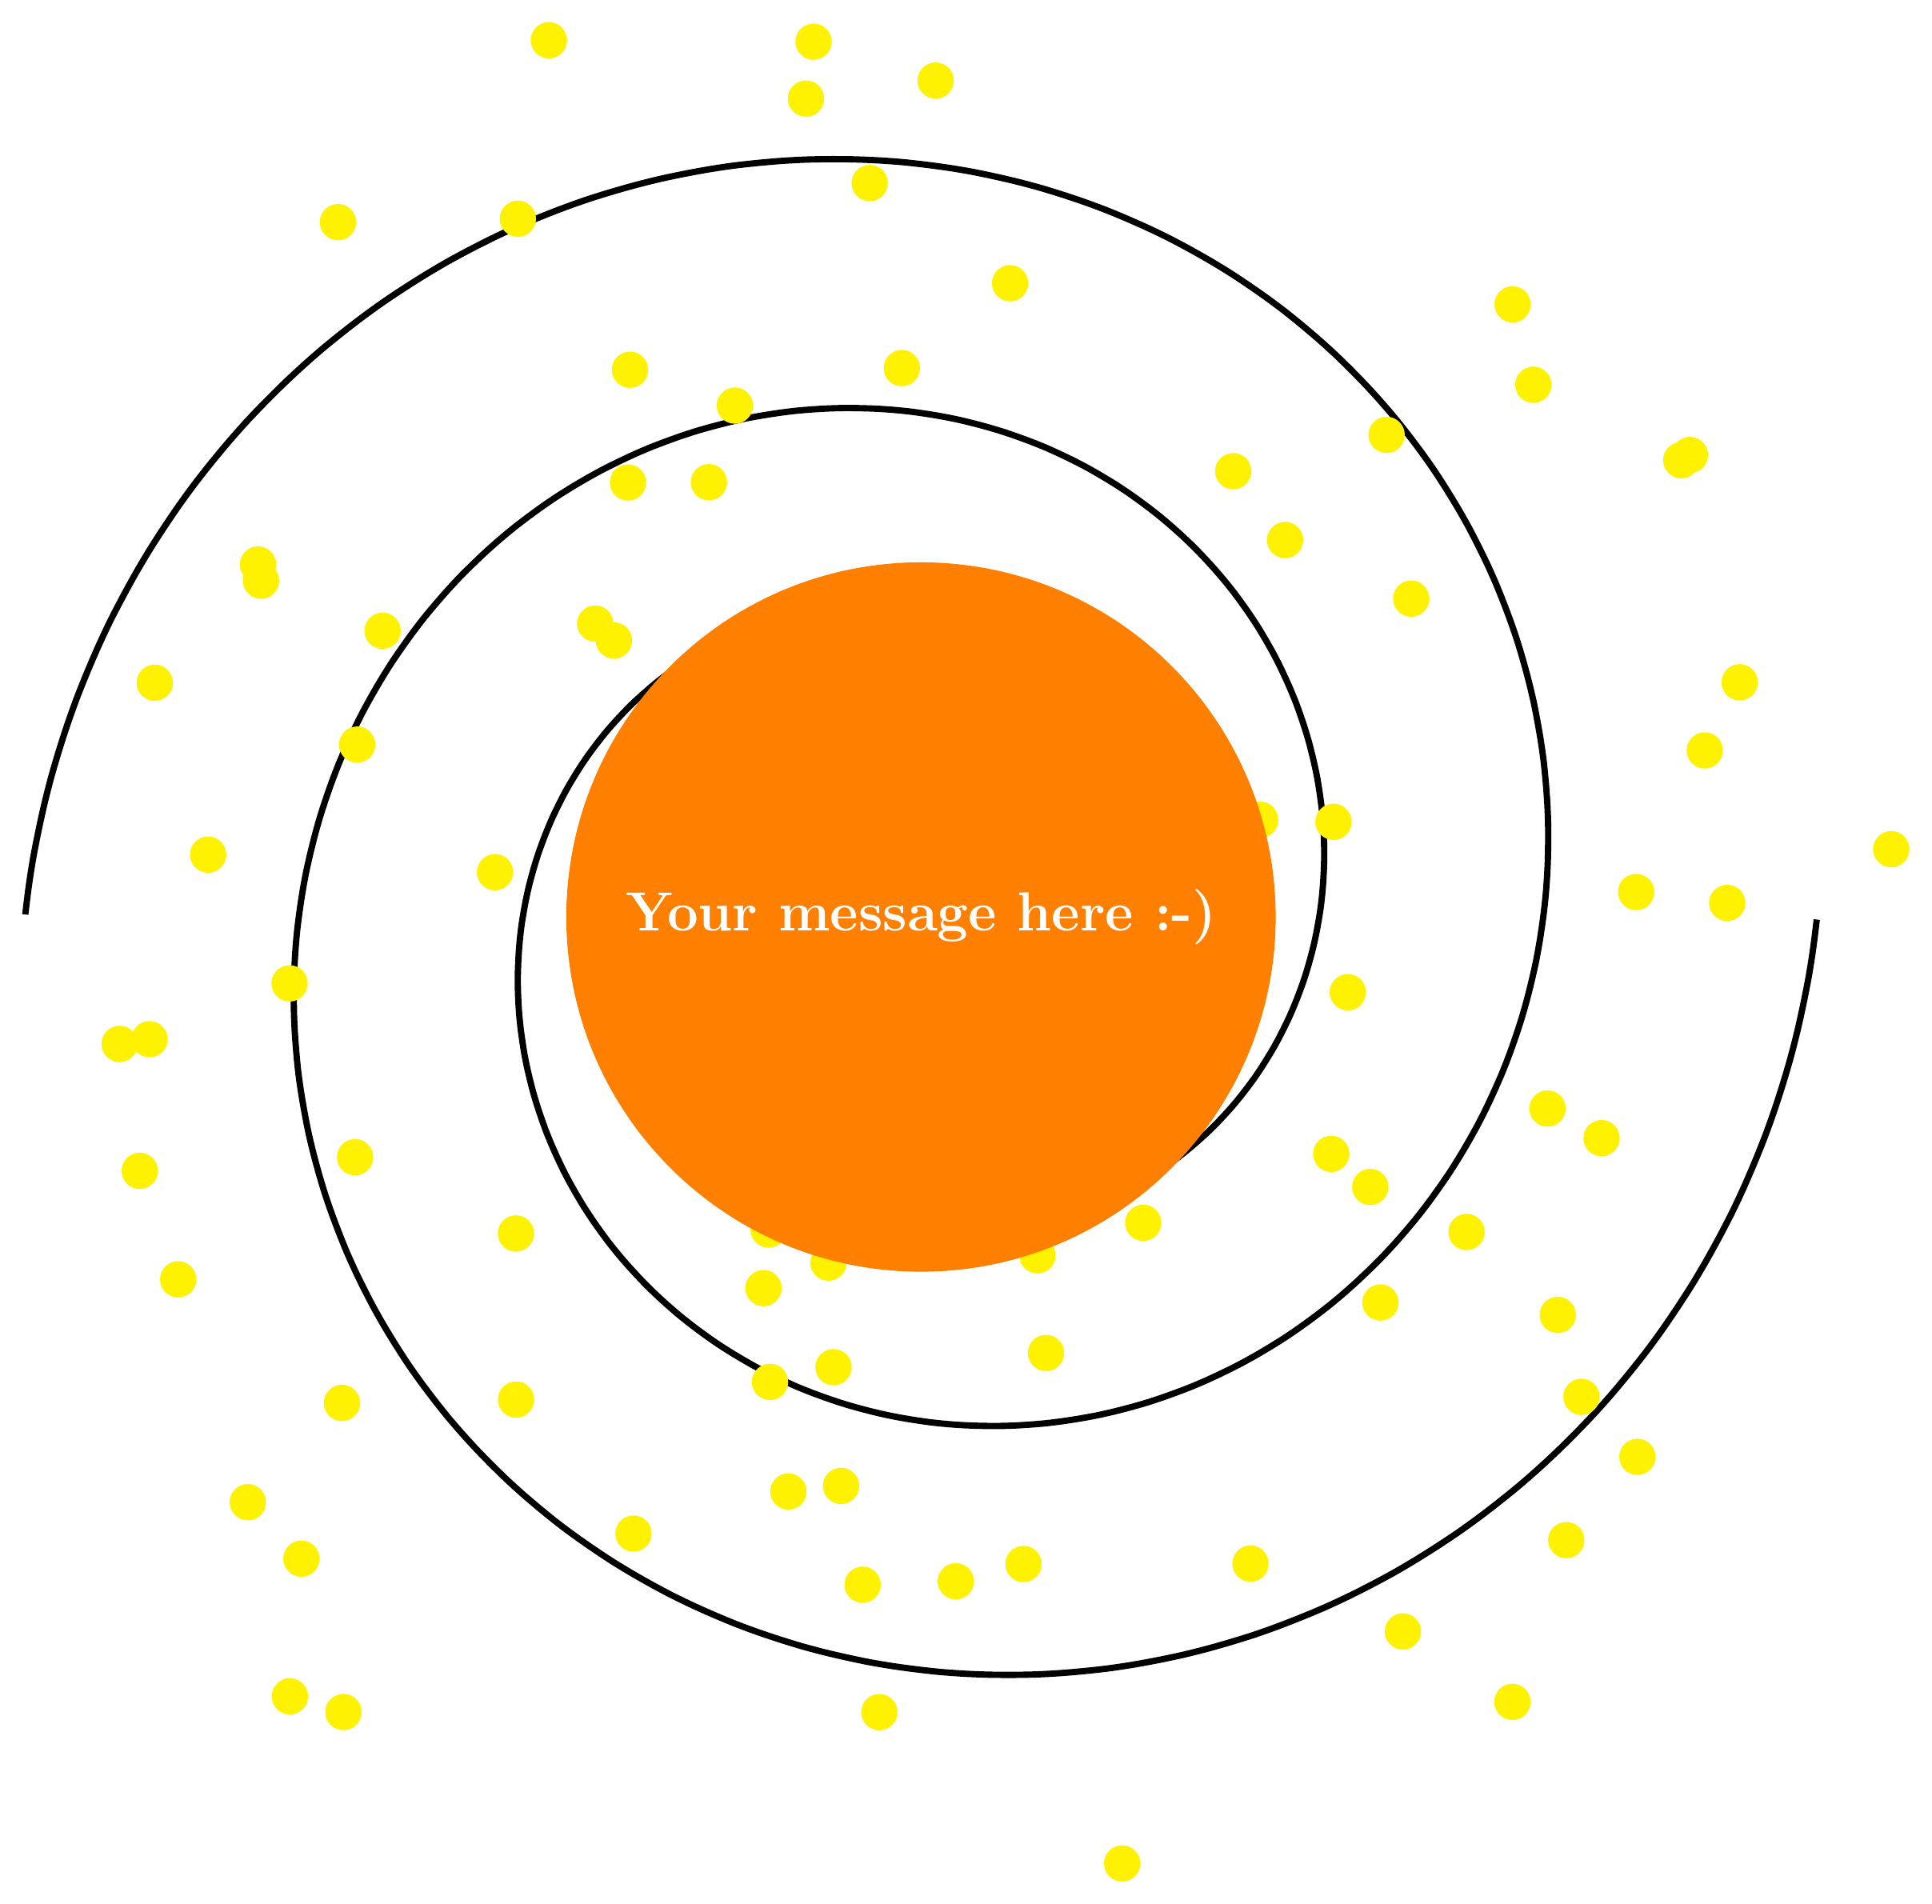
\begin{tikzpicture}[scale=8] % Scale up the entire picture

  % Draw spiral galaxy arms (increased thickness)
  \draw [black, line width=1mm, domain=0:6*pi, samples=600, smooth, variable=\t]
    plot ({\t r}: {0.005*\t*\t});
  \draw [black, line width=1mm, domain=0:6*pi, samples=600, smooth, variable=\t]
    plot ({\t r}: {-0.005*\t*\t});

  % Sprinkle stars (increased size)
  \foreach \i in {1,2,...,100}{
    \tikzmath{
      \angle = random(0,360);
      \radius = random(20,200)/100;
      \x = \radius*cos(\angle);
      \y = \radius*sin(\angle);
    }
    \filldraw [yellow] (\x,\y) circle (1pt); % Larger stars
  }

  % Galactic core (increased size)
  \filldraw [orange] (0,0) circle (20pt); % Larger core

  % Add text
  \node at (0,0) [white, font=\bfseries\Huge] {Your message here :-)};
\end{tikzpicture}
\end{document}
